\documentclass{article}

% Language setting
% Replace `english' with e.g. `spanish' to change the document language
\usepackage[ngerman]{babel}
% Set page size and margins
% Replace `letterpaper' with`a4paper' for UK/EU standard size
\usepackage[letterpaper,top=2cm,bottom=2cm,left=3cm,right=3cm,marginparwidth=1.75cm]{geometry}
% Useful packages
\usepackage{amsmath}
\usepackage{graphicx}
\usepackage[colorlinks=true, allcolors=blue]{hyperref}

\usepackage[utf8]{inputenc}
\usepackage{xcolor}
\usepackage{graphicx}
\usepackage[style=numeric, backend=biber]{biblatex}
\usepackage{fvextra}
\usepackage{csquotes}
\usepackage{svg}
\usepackage{amsmath}
\usepackage{datetime}
\usepackage{hyperref}
\usepackage[font={small,it}]{caption}
\usepackage{acronym}
\usepackage{listings}
\usepackage[T1]{fontenc}
\usepackage{subfig}

\usepackage{CJKutf8}

\usepackage{amssymb}
\usepackage{pifont}
\usepackage{wasysym}

\usepackage{tikz}
\usepackage{tkz-euclide}
\usetikzlibrary{automata, positioning, arrows}

\usepackage{pgfplots}

% example texts
\usepackage{blindtext}
\usepackage{lipsum}

% Table
\usepackage{tabularx}
\usepackage{longtable}

\usepackage{fancyhdr}
\usepackage{minted}
\newcommand{\newparagraph}[1]{\paragraph{#1}\mbox{}\\\\}
\renewcommand{\listfigurename}{Abbildungsverzeichnis}
\providecommand*{\listingautorefname}{Quellcode-Ausschnitt}

\renewcommand{\listoflistingscaption}{Quellcodeverzeichnis}
\renewcommand\listingscaption{Quellcode-Ausschnitt}
\setlength\headheight{16pt}
\pgfplotsset{compat=1.18}

%\pdfcompresslevel=0
%\pdfobjcompresslevel=0

\addbibresource{0.bib/bib.bib}

\title{Design und Implementierung eines Resource Management Games}
\author{Justin Nicola, Mat. 35441124, Informatik PO2018}

\begin{document}


% Begin Deckblatt
\thispagestyle{empty}

% Seminardaten
\begin{flushleft}
	Universität Kassel \hfill \today \linebreak
	Fachgebiet Gender/Diversity \linebreak
	Exposé Bachelorarbeit \linebreak
	Sommersemester 2022 \linebreak
\end{flushleft}

\vfill

% Titel
\begin{center}
	{\Huge \bfseries Bachelorarbeit} \\[12pt]
	{\huge Design und Implementierung eines Resource-Management-Games} \\[24pt]
	{\Large \bfseries Justin Nicola}
\end{center}

\vfill
\vfill

% persönliche Daten
\begin{flushleft}
	Justin Nicola \linebreak
	\href{mailto:065369@student.uni-kassel.de}{065369@student.uni-kassel.de} \linebreak
	Matrikelnummer: 35441124 \linebreak
	8. Fachsemester \linebreak
	Studienfach: Informatik, PO2018
\end{flushleft}

% End Deckblatt


\section*{Glossar}

%\begin{tabularx}{0.8\textwidth} { 
%    | >{\raggedright\arraybackslash}X 
%   | >{\centering\arraybackslash}X 
%    | >{\raggedleft\arraybackslash}X | }
%   \hline
%   Game Engine & Ein Framework zur Erstellung und Entwicklung von Computerspielen \\
%   \hline
%  \hline
%  \end{tabularx}


\maketitle
\section{Einleitung}

Bereits seit dem Jahr 1964 existieren Ressource Management Games. Das erste verzeichnete Spiel trägt dem Titel \glqq The Sumerian Game\grqq, wurde entwickelt von Mabel Addis und spielt in dem antiken sumerischen Stadtstaat Lagash \cite{rmgwiki}. Die Aufgabe des Spielers war es, in drei verschiedenen Segmenten mit jeweils eigenen Runden, die Bevölkerung und die Ressourcen so anzuordnen, dass ein erfolgreiches Überleben der Einwohner gesichert ist, trotz zufälliger Katastrophen oder Events. Seitdem hat sich in der Branche des Game Developments und der Kategorie der Ressource Management Games einiges getan, von SimCity über Anno, bis hin zu RimWorld oder Factorio. Es gibt verschiedenste Unterkategorien von Ressource Management Games, welche alle eigene Siegbedingungen, Tücken und Eigenschaften besitzen, wie auch typische UI-Elemente und -Anordnungen. Die Branche ist erfolgreicher denn je und erfreut sich stetigem Wachstum, doch die Frage ist, in welche Richtung werden sich Ressource Management Games entwickeln? Gibt es zurzeit Optimierungsbedarf an bestimmten Stellen? Was hält den Spieler dazu an, weiter das Spiel zu spielen, und wie kann man den Spaß optimieren? Was sind gängige Ressourcen, und was eher untypische? Gibt es eine (bisher) minimale und maximale Komplexität?


\section{Beispiele}
Um einen Überblick der Entwicklung und der Grundlage des Genres zu verschaffen werden im Folgenden einige Beispiele genannt, kategorisiert als Klassiker und Neuerscheinungen. Anhand dieser Beispiele wird anschließend eine Analyse durchgeführt, die den IST-Zustand abbilden soll.

\section{Analyse}
Im Folgenden wird eine IST-Analyse des Spiels \textit{RimWorld} durchgeführt, um anhand eines Colony Management Games herauszufinden, welche Mechaniken und Eigenschaften dieses Spiel auszeichnen, und welche davon gegebenenfalls übernommen werden könnten für den Prototyp eines neuen Spiels. Dazu wird zu aller erst das Spiel näher untersucht, darunter die Mechaniken, die Kernelemente und das User-Interface. Anschließend werden Leitfaden-Interviews durchgeführt, dessen Ergebnisse und Transkripte verwendet werden, um Hypothesen für den Prototypen aufzustellen. Diese Hypothesen werden letztendlich mit einer Umfrage geprüft und mit der Implementierung des Prototypen schlussendlich umgesetzt. 


\begin{figure}
    \begin{center}
        
\includegraphics[width=400px]{0.bilder/interviewphases.png}
    \end{center}
    \caption{Die Vier Phasen des Interviews} \label{image:interviewphases}
\end{figure}
\subsection{Interviews}
Für die Ermittlung gut funktionierender Mechaniken und Konzepte wird auf die Methode des kontextuellen Interviews zurückgegriffen \cite*[]{holtzblatt_beyer_1997}. Dazu wird ein Leitfadeninterview angefertigt, um qualitative Daten von den Teilnehmern zu extrahieren und daraus Hypothesen anzufertigen \cite*[]{baur_blasius}. Nachdem die Hypothesen erarbeitet wurden, werden diese mittels einer Umfrage in einem breiten Umfang überprüft. Es werden drei Personen ausgewählt, wobei die Erfahrung aller Personen in Bezug auf das Spiel und das Genre generell variiert. Diese Personen, im Folgenden auch \textit{Probanden} genannt, werden in Einzelgesprächen dazu gebeten, dass Spiel eine Stunde lang zu spielen. Einzelgespräche beziehungsweise -interviews sind Gruppengesprächen vorzuziehen, da die einzelnen Probanden einen entspannteren Zeitplan haben, sich gänzlich auf das Spiel und die Fragen fokussieren können und keine Gefahr laufen, abgelenkt zu werden oder mit anderen Probanden in Gespräche zu gelangen \cite*[]{lankoski_bjork}. Das Interview gliedert sich in vier Phasen (vgl. \autoref{image:interviewphases}):
\subsubsection{Einleitung}
Um die erhobenen Daten richtig kategorisieren zu können, werden als erstes grundlegende Daten zu der Person an sich erfasst:
\begin{itemize}
    \item F1: Wie alt bist du?
    \item F2: Nach welchem Geschlecht identifizierst du dich?
\end{itemize}

\subsubsection{Aufwärmen}
Im zweiten Schritt des Interviews werden etwas spezifischere Fragen zu der Erfahrung und dem Verhalten bezüglich Videospielen gestellt:
\begin{itemize}
    \item F3: Hast du bereits Erfahrung in Videospielen?
    \item F4: Hast du bereits Erfahrung in Resource Management Games?
    \item F5: Hast du RimWorld bereits zuvor gespielt?
    \item F6: Bevorzugst du Konsole oder Computer?
    \item F7: Bevorzugst du Controller oder Tastatur und Maus?
\end{itemize}

\subsubsection{Beobachtung}
Die Phase der Beobachtung beschreibt die Spielphase. Der Proband wird aufgefordert, das Videospiel \textit{RimWorld} zu spielen. Es ist von fundamentaler Wichtigkeit für diese Phase, das die beobachtende Person keinerlei Versuch unternimmt, sich in das Spielgeschehen oder das Verhalten der beobachteten Person einmischt. Es wird auch unterlassen, begangene Fehler aufzuklären oder in irgend einer anderen Art und Weise zu helfen. 

\begin{itemize}
    \item F8: Welche Emotion wird gerade verspürt?
    \item F9: Ist das Spiel für den Probanden immersiv?
    \item F10: Hat der Proband Verlustängste bezüglich der Kolonisten?
    \item F11: Wieso machst du \_\_\_?
    \item F12: Weißt du, was du nun tun kannst?
    \item F13: Was ist dein nächstes Ziel?
    \item F14: Verwendet der Proband die Prioritätenliste?
    \item F15: Kommt der Proband gut mit der indirekten Anweisungsmechanik zurecht?
\end{itemize}

\subsubsection{Abschluss}
In der Abschlussphase wird der Proband gebeten, eine eigene Meinung abzugeben. Außerdem können Fehler aufgeklärt werden und inhaltliche Fragen beantwortet werden, ohne dass sie nun das Verhalten im Spiel verzerren.

\begin{itemize}
    \item F16: Was hast du als gut empfunden?
    \item F17: Was hast du als schlecht empfunden?
    \item F18: Wie findest du das indirekte Anweisen?
    \item F19: Was sagst du zu der Ressourcenvielfalt?
    \item F20: Was hältst du von dem Prioritätensystem?
    \item F21: Wie findest du die vielen zufällig generierten Umstände?
\end{itemize}


\subsection{Umfrage}
Die zuvor erarbeiteten Hypothesen werden im Folgenden über die empirische Methode der Online-Umfrage überprüft \cite*[]{Evans2005TheVO}.  Die Online-Umfrage wird auf \textit{Discord}-Servern durchgeführt. Discord ist ein soziales Medium, welches dazu dient Videos oder Videos auszutauschen, oder sich über Sprach- oder Textkanäle miteinander zu vernetzen und zu kommunizieren \cite*[]{discord:usage}. Discord hat 140 Millionen aktive Nutzer pro Monat, Tendenz stark steigend (Stand 2021) \cite*[]{discord:statistics}. Es gibt dabei mehrere \textit{Discord Server}, welchen man mit einer Einladung beitreten kann, auf welchem sich mehrere Personen befinden, mit welchen man kommunizieren kann. Es gibt für RimWorld einen dedizierten Discord Server, auf welchem sich (Stand 15.08.2022) 37.634 Mitglieder befinden.

\section{Prototyp}
Für den praktischen Anteil dieser Arbeit wird auf Grundlage der gewonnenen Erkenntnisse aus Sektion 3 ein Prototyp angefertigt. Es wird also auf die Hypothesen zurückgegriffen, welche durch die Interviews und Umfragen erarbeitet und überprüft wurden. 

\subsubsection{Thematik}
Für den Prototypen bedarf es einer Thematik beziehungsweise einer Idee für das Gesamtkonzept. Dafür wurde die Idee einer \textit{Bienenkolonie} für interessant befunden. Bienen und deren Kolonien sind aus vielerlei Hinsicht geeignet als Thematik für den Prototyp, darunter der Fakt, dass Bienen bekannt dafür sind, Honig zu produzieren, wobei Honig eine konkrete Ressource darstellt. Im Kontext eines Resource Management Games und mit Rücksicht auf das zuvor untersuchte Spiel \textit{RimWorld} eignet sich jedoch am besten eine ganz spezifische Art der Bienen, die \textit{Honigbiene}, genauer gesagt die \textit{Westliche Honigbiene} (lat. \textit{apis mellifera}) \cite*[]{bees:name}. Grund dafür ist die Verhaltensweise von Honigbienen, da diese, anders als nahe Verwandte, stärker dazu tendieren, in Kolonien zu leben. Hummeln beispielsweise formen zwar auch Kolonien, aber deutlich kleinere und kürzer lebende. Die meisten Arten der Wildbienen jedoch sind tendenziell Einzelgänger. Eine weibliche Wildbiene legt ein Nest und versorgt ihren Nachwuchs mit Pollen und Nektar \cite*[]{bees:wild}. Somit bietet die Gattung der Honigbiene einige Vorgänge, welche sich in ein Colony Management Game umsetzen lassen. Dazu werden im Folgenden interessante Vorgänge und Eigenschaften der Gattung der Honigbiene genauer untersucht.

\newparagraph{Nahrung}
Eine Honigbiene ernährt sich primär von \textit{Nektar}, welchen sie von Blumen sammelt. Dieser Nektar ist zuckerhaltiger Saft, welcher von den Pflanzen ausgeschieden wird, um damit Insekten verschiedener Arten anzulocken. Dabei sind Sonnenblumen, Obstblüten, Löwenzahn und Raps besonders gute Nektarquellen \cite*[]{bees:food}. Eine weitere Möglichkeit um an energiereichen Zucker zu gelangen ist der sogenannte \textit{Honigtau}, welcher von einigen Insekten, darunter Blatt- und Schildläusen, ausgeschieden wird. Aus diesen beiden zuckerhaltigen Säften können die Bienen den \textit{Honig} produzieren, welcher ebenfalls als Nahrungsquelle dient, aber vor allem über die Wintermonate besonders wichtig ist, da Honig sehr lange haltbar ist \cite*[]{bees:honeywinter}. Der durch Honigtau produzierte Honig wird von Imkern als \textit{Waldhonig} gekennzeichnet \cite*[]{bees:food}. Saugt eine Biene den Nektar einer Blüte auf, gelangt dieser in den \textit{Honigmagen}. Dort kommt er in Kontakt mit verschiedenen Enzymen, welche den Nektar in \textit{Glukose} (Traubenzucker) und \textit{Fruktose} (Fruchtzucker) \cite*[]{bees:glucosefructose} aufspalten. Diesen biochemisch veränderten Nektar gibt die \textit{Sammelbiene} im Bienenstock an die sich dort befindlichen \textit{Arbeitsbienen} durch Auswürgen weiter, welche den Nektar erneut aufnehmen und auswürgen. Mit jedem dieser Prozesse wird der Nektar viskoser, wodurch allmählich Honig entsteht \cite*[]{bees:nectartohoney}.

Neben dem Nektar, dem Honigtau und dem Honig, welche primär als Quellen für Kohlenhydrate dienen, benötigen Bienen außerdem noch Quellen für Fette und Proteine. Dafür werden \textit{Pollen} verwendet, wobei Pollen die männlichen Geschlechtszellen einer Samenpflanze sind. Da die Samenpflanze mehr Pollen produziert, als für die Fortpflanzung nötig, können diese ohne Probleme von den Sammelbienen aufgenommen werden \cite*[]{bees:honeywinter}. Die Pollen werden in \textit{Pollenpaketen} aufbewahrt (vgl. \autoref{image:pollenpaket}), wobei Teile der aufgesammelten Pollen nicht in diesen Pollenpaketen landen, sondern an den Hinterbeinen haften bleiben. Besucht diese Sammelbiene nun eine weitere Blüte, werden diese Pollen abgestreift und der Fortpflanzungsmechanismus der Samenpflanze profitiert. Besonders pollenreiche Quellen sind dabei Obstbäume, Mohn, Mais, Klee und Raps \cite*[]{bees:honeywinter}.

\begin{figure}
    \begin{center}
        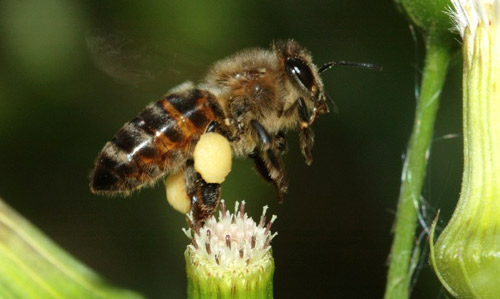
\includegraphics[width=300px]{0.bilder/pollenpaket.jpg}
    \end{center}
    \caption{Pollenpakete einer Honigbiene (\cite{bees:name})} \label{image:pollenpaket}
\end{figure}

Die letzte wichtige Ressource, welche Bienen für ihr Überleben benötigen, ist Wasser. Dieses kann von Flüssen oder Seen bezogen werden, wobei diese Quellen nicht mehr als 500 Meter weit vom Stock entfernt sein sollten. Erhalten Bienen nicht genug Wasser, können diese unter Verstopfungen leiden, was für das Überleben gefährlich sein kann \cite*[]{bees:honeywinter, bees:food}.

Es lassen sich somit wichtige Ressourcen identifizieren: \textit{Nektar, Honigtau, Honig, Pollen} und \textit{Wasser}. Außerdem ist die Aufteilung zwischen \textit{Sammel-} und \textit{Arbeitsbiene} eine mögliche Mechanik. Die Umwandlung von Nektar und Honigtau zu Honig könnte ebenfalls eine Mechanik darstellen, wie auch die naturgegebenen Quellen für Nektar, Honigtau und Pollen.

\newpage
\printbibliography

\newpage
\section*{Notizen}
\subsection*{Offene Fragen}
\begin{itemize}
    \item Age of Empires und Civ noch ausbauen?
    \item Genauer auf alle Nachfolger und Vorgänger eingehen, mit Publishern, Developern und Änderungen?
    \item Wirklich alle verfügbaren Rezensionen suchen und reinpacken?
    \item Umfrage zu gespielten Klassikern über Discord?
    \item Noch Anno 1602 als Klassiker hinzufügen?
    \item Notable Mentions? Cruisader Kings, Anno 1602, 
\end{itemize}

\subsection*{Ideen}
\begin{itemize}
    \item HexaBees turn based, oder RTS?
    \item Falls RTS dann 
\end{itemize}

\subsection*{Fremdwörter}
\begin{itemize}
    \item Game engine
    \item Real Time Strategy
    \item launch arcos
    \item Singeplayer (Game)
    \item Isometrisch
    \item Domination
    \item Space Race
    \item 
\end{itemize}

\subsection*{Abkürzungen}
\begin{itemize}
    \item SAT - Sega Saturn, Konsole
    \item RTS
    \item R - Residents
    \item C - Commercial
    \item I - Industries
    \item KI
    \item 
\end{itemize}
\end{document}